%!TEX root = ../main.tex

\chapter{Implementation}

\label{Chapter3-implementation}

In this chapter, we will first discuss some common high-level design decisions that apply to all of our implementations.
Following this, we will delve into the specifics of each key-value (KV) store, including their internals and implementation details.
Lastly, we will demonstrate how we leveraged log-structuring to achieve the desired incremental snapshotting capability of our key-value store.

\section{Common design decisions}

\subsection{Application Programming Interface}

Firstly, we designed our implementations to expose a common interface (API) to the programmer.
This allows for easy benchmarking, testing, and ultimately a fair comparison between the engines.
The API is programmatically defined within a parent class that is inherited and extended by the classes corresponding to each engine, of which the exact method signatures can be found in appendix \ref{Appendix-A-code}.
The methods supported are:

\begin{itemize}
    \item \verb"get": For retrieving the value of a given key. This operation is called a \textit{read}.
    \item \verb"set": For setting the value of a given key. If the key does not exist, it is inserted in the database with the given value, and if it already exists it is updated to the given value. If the value is empty, this is considered a delete. We refer to all these operations as \textit{writes}.
    \item \verb"close": Closes the database by flushing all buffers and closing all files.
    \item \verb"snapshot": Takes a snapshot of the current state, by flushing all buffers and pushing the latest created files to a remote directory (more on that in section \ref{section-replicas}).
    \item \verb"restore": Using the remote directory, it pull all files  associated with a given version, restoring the state of a specific point in time when a snapshot was taken.
\end{itemize}

The decision for deletes to be just writes to empty values was taken because it greatly simplifies both usage and implementation. The user does not have to call special methods, and on the side of the implementation, we avoid dealing with intricacies like ``tombstones'' - special markers popular in many databases (like [\cite{myrocks}]).

Also, all keys and values are in the form of raw bytes.
This is also the design decision followed in the APIs of major commercial key-value stores like \cite{rocksdb} and \cite{redis}, because besides offering simplicity, it also allows for maximum flexibility, as any other data type can be serialized in bytes and makes the encoding of the key-value pairs on disk easy.

Regarding the encoding of the key-value pairs on disk, we encode each key-value pair as shown in figure \ref{fig:encoding}: we first encode the length of the key in bytes, then we write the key itself, and then we repeat the same for the value. This enables us to avoid any kind of escaping and special characters. Additionally, each key-value store accepts as arguments in the constructor the maximum key length and the maximum value length, which we use to determine the amount of bytes we will use for the encoding.

\begin{figure}[h]
    \centering
    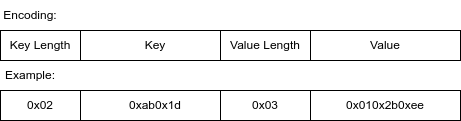
\includegraphics[width=0.8\textwidth]{encoding.png}
    \caption{Encoding \& Example.}
    \label{fig:encoding}
\end{figure}

Another design decision is to store all data in files under one directory on disk, which enables easy backups and management in general. Upon startup, a key-value store will attempt to fetch the latest snapshot, if it has been initiated with a connection to a remote source (either a path in the same machine, which is expected to have been mounted remotely elsewhere, or \textit{minio}, more on that in section \ref{section-replicas}). If a key-value store is not connected to a remote directory, and finds data in its local data directory from a previous run, it will rebuild its indices from this data.

% TODO mention how the encoding allows us to have keys and values of arbitrary size and we dont need to address the log as an array? see also hybridlog for that.
% also this encoding is called length encoding...mention that as well

\section{Log-Structured Merge-Tree}

% maybe move these to related work??

The Log-Structured Merge-Tree (LSM-Tree) is a disk-based data structure [\cite{lsmtree}], and one of the most prominent, battle-tested, and well-researched key-value store backend engines.
It was invented by Patrick O'Neil in 1996 and has since been used in multiple databases, such as Google's LevelDB [\cite{leveldb}], Meta's RocksDB [\cite{rocksdb}] and Apache's Cassandra [\cite{cassandra}].

The LSM-Tree makes extensive use of the \textit{log-structuring} technique, which first appeared in the LFS file system [\cite{lsm-filesystem}] and has since been used not only in LSM-Tree-based database management systems, but also in other types of storage engines, even B-Tree-based ones [\cite{llama}].

Log-structuring offers significant speedups by significantly reducing the number of writes per page and transforming them into a "sequential" format.
In other words, it consolidates numerous random writes into a single large multi-page write [\cite{llama}].

In this work, we use log-structuring extensively, because, besides its advantages in I/O operations, it also provides a straightforward way to create incremental snapshots of the database's state.
We analyze the way we leveraged log-structuring for incremental snapshotting later, in section \ref{section-incremental-snapshots}.

Given the close relationship between log-structuring and the LSM-Tree (which makes extensive use of it), we will introduce the concept in tandem with the LSM-Tree.

\subsection{Design}
\label{subsection-lsm-design}

The power of the LSM-Tree can be partially attributed to the fact that it uses lightweight indices, when compared to B-trees which effectively double the cost of every I/O operation to maintain their indices [\cite{lsmtree}].
This enables the LSM-Tree to scale to very high write and read rates.

However, one other important factor for the LSM-Tree's fast I/O is the use of an in-memory buffer, also called \textit{memtable}, which aggregates the updates and when it's full, it flushes them to disk sequentially.
As it is well known, disks perform much faster sequential operations that operations than require random-access, especially in the cloud, where inexpensive disks have limited I/O rates [\cite{llama}].

This buffer flushes the aggregated data into \textit{sorted} chunks of data that are commonly referred to as SSTs for ``Sorted String Tables'', but we will just call them ``runs''.
Sorting is essential for indexing, as it enables us to lookup keys in logarithmic time.

So, initially, as we are writing data, we keep them in our buffer, and when this buffer is full, we flush it into a run-file. This can be seen in figure \ref{fig:lsm.flush}, where the file \verb"L0.0.run" is created, corresponding to the first file of the first run - everything is zero-indexed.

\begin{figure}[h]
    \centering
    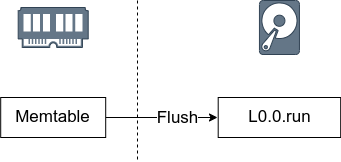
\includegraphics[width=0.6\textwidth]{lsm.flush.png}
    \caption{LSM-Tree flushing.}
    \label{fig:lsm.flush}
\end{figure}

As we continue writing key-value pairs, we create new runs in the same level by flushing our memtable, until their number reaches the maximum allowed runs per level, which is defined by the parameter \verb"max_runs_per_level" when instantiating the LSM-Tree. When that happens, a merge is triggered; the merge will merge these files into one file in the next level, and will check if the number of runs in that level is equal to the maximum runs per level. If it is, it will cascade the merging recursively to the next level, and this process will keep happening until no merges need to be done. The merging process is shown in figure \ref{fig:lsm.merge}, where the runs in the first level are merged into \verb"L1.0.run". After being merged, the files in the first level are deleted. 

\begin{figure}[h]
    \centering
    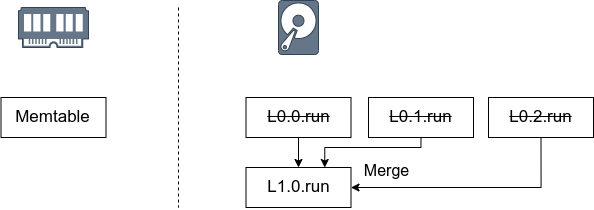
\includegraphics[width=0.8\textwidth]{lsm.merge.png}
    \caption{LSM-Tree merge.}
    \label{fig:lsm.merge}
\end{figure}

The merging process resembles the greedy merging step in the mergesort algorithm, because every run is sorted. We keep a number of file descriptors equal to the number of runs we are merging, and go through all of them at the same time. We take care to write the smallest key first, to make sure that the resulting merged file is also sorted. In case of two or more conflicting keys during the process, we write the latest one (the one with the largest run index) and skip the rest, as those have been overwritten by a more recent write and are not valid anymore. This is also how the LSM-Tree performs garbage-collection - during the merging process, invalid values are dropped.

To retrieve values using the \verb"get" operation, it is necessary to search through the files in reverse order to locate the latest write.
This involves performing a binary search on each file, starting from the first level, and then searching within each level from the runfile with the highest index to the lowest.

This search can be time-consuming if done on the files themselves, because it would involve a large number of I/O operations, so we use a data structure called \textit{fence pointers} [\cite{fence-pointers}] to speed up the process. The fence pointers are essentially arrays that allow us to do binary-search in memory, and associate a key with its offset in the runfile. Of course, they don't store all the keys, as that would be like keeping all the keys in memory and thus we would miss one of the main points of using an LSM-Tree. Instead, we use a subset of them, and since the runfile is itself sorted, if the key we are looking for does not have a fence pointer itself, we still know the offsets among which it should be (hence the name ``fence pointers'') and we can go ahead and search for it linearly on the file. The gap in numbers of key-value pairs between the offsets of the pointers is controlled via a parameter called \verb"density_factor" - the higher its value, the greater the gaps and the more key-value pairs we have to search sequentially on disk.

The fence pointers offer a significant speedup, but we can skip entire runfiles if we know for sure that they don't contain the key we are looking for by using Bloom filters [\cite{bloom-filters}]. The Bloom filter is a probabilistic data structure that when queried if a key exists in a set (a runfile in our case) it will answer negatively with 100\% certainty if it does not. The positive answer is not always accurate, but having a few false positives is no problem for files that we were going to search anyway if we didn't have the Bloom filter.

After these additions, value retrieval looks as follows (see figure \ref{fig:lsm.get}): starting from the first level and from the rightmost (latest) run, we query the Bloom filters for the key we are looking for. When a Bloom filter answers positively, we query the fence pointers, and get an offset. We look up at most $d$ key-values in that file following this offset, where $d$ equals the density factor. If the key is not found, we repeat this process with the next runfile. If we exhaust the lookups and haven't found the key, we return the empty value (0 bytes).

\begin{figure}[h]
    \centering
    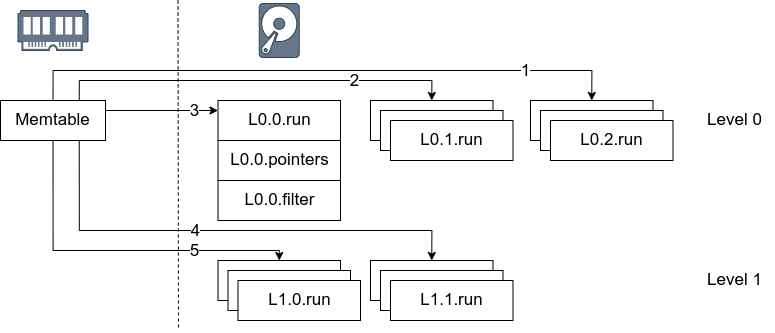
\includegraphics[width=0.8\textwidth]{lsm.get.png}
    \caption{LSM-Tree value retrieval.}
    \label{fig:lsm.get}
\end{figure}

\subsubsection{Tiering vs Leveling}

LSM-Trees come in two flavors, depending on the merging strategy: there are the LSM-Trees that use \textit{tiering} and those that use \textit{leveling} [\cite{compactionary}]. In tiering, we use up to $R$ runs per level, while in leveling we only use one.
As we increase $R$, the first level essentially transforms into an append-only log, which has the highest write speed. However, the reads become slower, as the LSM-Tree has to search a higher number of files to retrieve a value. On the other hand, in leveling when $R=1$, the LSM-Tree merges each file directly to the runfile of the next level, using the file sizes as thresholds that trigger merges. This optimizes the read performance but impedes the writes [\cite{lsm-design-space}].

Our implementation uses tiering because we are optimizing for writes. Nonetheless, the $R$ value described above is still configurable, and we will analyze the performance of the LSM-Tree for various values of it in Chapter \ref{Chapter4-evaluation}.

\subsection{Implementation}

As we stressed in the previous subsection, the properties of the LSM-Tree are derived primarily from having \textit{sorted} runfiles.
To remove the values from the memtable when flushing it in order, we need a data structure that does this operation efficiently.
% i can write this a bit better...
At the same time, we want this data structure to support efficient lookup and insertion/update of values.
These requirements are satisfied by Skip lists, or self-balancing binary-tree structures, like AVL trees and Red-Black trees. The skip list is used in some commercial LSM-Tree-based key-value stores, like \cite{leveldb} but operations on them are not guaranteed to be efficient due to their probabilistic nature. On the other hand, AVL trees and Red-Black trees have guaranteed access, lookup, insertion, and delete complexity of $\mathcal{O}(\log{}(n))$.

In our implementation, we used the \verb|sortedcontainers| package, a Python implementation of an associative array which offers the same complexity for the above operations.

For the fence pointers, we used the same package. We use JSON to serialize them and store them to disk, and when we want to load them in memory, we read the JSON file, rebuild the sorted container and keep it in memory to serve queries.

For the bloom filters, we could not use the most popular publicly available implementation due to a versioning incompatibility so we implemented it. We serialize and deserialize it using JSON as well, with base64 encoding for the Bloom filter's bitarray.

% TODO add details on how the bloom filter works

% TODO the write-ahead log!!!

% possible optimizations:
% 1. https://www.youtube.com/watch?v=b6SI8VbcT4w - dostoevski, monkey, wacky
% 2. fence pointers can be used to organize data into compressible blocks
% 3. the .filter and .pointers files could be embedded to the runfile (and then do a relative seek from the end)
% this would help with the save to replica things
% checksums? these are apllicable to all logstruct
% as well as compression
% per level bloomfilters, with a small memory increase
% fence pointer optimizations see 

\section{AppendLog}



\section{HybridLog}

\section{Replicas}
\label{section-replicas}

% possible extensions/optimizations applicable to all engines:
% concurrency! explain how it can be applied, what to lock etc.
% mmap for the files
% checksums for malformed records

\section{Incremental Snapshots}
\label{section-incremental-snapshots}
